\documentclass[11pt]{article}
\usepackage{amssymb}

\usepackage{fullpage,times,hyperref,hypcap,namedplus}
\usepackage{cite,enumitem,graphicx,amsmath}

\hypersetup{colorlinks=true,allcolors=black}

\title{\bf Fast clustering algorithms for points in an Euclidean space and its applications to Drop-Seq data}
\author{\bf Guilherme de Sena Brandine}
\date{\today}

\begin{document}

\maketitle

\section{Problem Statement}
Let ${\rm I\!R}^d$ be the $d$-dimensional euclidean space and $X = \{x_1 \dots x_n\} \subset {\rm I\!R}^d$ be a set of $n$ vectors in this space where the euclidean distance is naturally defined as $d(i,j) = \sqrt{(x_i - x_j)^T (x_i - x_j)}$, for which the inequality $d(i,j) \leq d(i,k)+d(k,j)$ is valid for all $i,j,k \in \{1,\dots,n\}$. We want to find a \emph {clustering function} $C:\{ 1 \dots n \} \rightarrow \{1 \dots K \} \cup \{ \Phi \}$ that assigns the $n$ points to $K \ll n$ categories (or possibly none) in such way that some penalty function $F(X,C)$ is minimized. For instance, a common choice for $F$ is the \emph{within cluster sum of pairwise distances} - which we'll call $F_w$ - given by:

\begin{equation}
F_w(X,C) = \alpha \mathop{\sum \sum}_{C(i)=C(j)\neq \Phi} d^2 (i,j) + \beta H(K)
\end{equation}

Where $H(K)$ is a non-negative increasing function that penalizes a large number of clusters in the dataset. Some clustering methods explicitly try to minimize the penalty function utilizing numerical methods, whereas others use heuristics and procedural methods that guarantees that the penalty is a sufficient approximation of the theoretical minima. For the specific practical problem of single cell RNA-Seq subpopulation discovery, a good clustering method has the following properties: \\
\\
1) The algorithm can find the optimal number of clusters without prior information\\
\\
2) The clustering method can discover outlier cells that do not belong to any cluster (noise cells). \\
\\
3) The \textbf{average} speed is sub-quadratic (as comparing pairwise distances is costly)\\
\\
4) Every element has a probability value assigned to every cluster.


\section{Clustering Algorithms}
Very few methods exist that satisfy all the 4 criteria (so far none that I'm aware of, especially because of condition 4), so here we study some which satisfy at least 3 of the 4. So far I only have two but I'll follow up with the other ones I find. 

\subsection{DBSCAN}
Density Based Spatial Clustering of Applications with Noise \cite{dbscan} is the currently used method in drop-seq datasets. The method takes two parameters as an input: $\epsilon$ and $K$. It first considers as noise points all of which have less than $K$ points within a distance of $\epsilon$ from it. It then builds a graph in which each point is connected to all the points in its $\epsilon$ neighborhood. The connected components in this graph - which can be found with a simple DFS - are the resulting clusters. \\
\\
\textbf{Advantages}: Querying the neighbors within a distance of $\epsilon$ can be easily retrieved using appropriate data structures such as KD-tree, and although the worst case is still $O(N^2)$ (for example if $K=N$, which would make no practical sense), in practice it can handle drop-seq clustering in a matter of minutes. \\
\\
\textbf{Disadvantages}: The performance of the method is highly dependent on the values of $K$ and $\epsilon$. One possible way to determine the value of $\epsilon$ that yields good results is to choose a small value of $K$ (usually $K=20$) and plot the sorted values of the $k-th$ nearest neighbor of each cell. Noise cells will have larger values of this distance, so a "knee" in such plot would give a good indication of a value of $\epsilon$


\subsection{OPTICS}
Ordering Points To Identify the Clustering Structure \cite{optics} is an improvement on DBSCAN that can find clusters of different densities as it is not influenced by the $\epsilon$ parameter after a certain threshold (it mostly changes runtime performance), and $K$ is set to be the minimum cluster size to be considered. \\
\\
The algorithm outline is to keep track of two values for core points: Its distance to its $K$-th nearest neighbor and its smallest radius that makes it reachable from a core point $q$. The maximum of these two values is called its \emph{reachability distance} and every point's reachability can be found by DFS-ing through the $K$ nearest neighbors graph, after which a point hierachy is generated and a cutoff can be set to define noise points and clusters. The algorithm runs in $O(N W logN)$, where $W$ is the average number of neighbors in the $\epsilon$ radius, so if $\epsilon$ is small enough its speed is still acceptable. 
\begin{figure}[h]
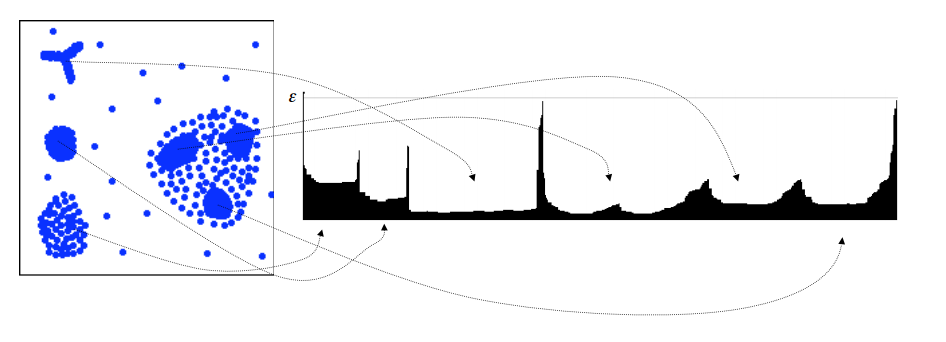
\includegraphics[scale=0.5]{OPTICS}
\caption {Reachability distances ploted by DFS-ing through the graph. The clusters are are generated by intersecting a horizontal line on some height $\epsilon' < \epsilon$}
\end{figure}

\section{Data Visualization}
\subsection{ZIFA}
Zero Inflated Factor Analysis \cite{zifa} is a dimensionality reduction technique that takes into account the drop-out rates. The user defines the number of dimensions $K$ and the data is assumed to come from a latent $N \times K$ matrix ($K \ll D$) and it assumes the observed matrix $Y$ is drawn independently through the following steps:

\begin{equation}
\begin{split}
z_i \sim Normal(0,I) \\
x_i | z_i \sim Normal (Az_i + \mu, W) \\
h_{ij} | x_{ij} \sim Bernoulli ( p_0 ) \\
y_{ij} = 
\left\{
\begin{array}{ll}
x_{ij}\mbox{ if }h_{ij}=0\\
0 \mbox{ if } h_{ij}=1
\end{array}
\right.
\end{split}
\end{equation}

Where $I$ is the $K \times K$ identity matrix, $A$ is a $D \times K$ factor loading matrix, $H$ is a $D \times N$ masking matrix, $W = diag ( \sigma _{1}^{2}, \dots , \sigma _{D}^{2} )$ is a $D \times D$ diagonal matrix and $\mu$ is a $D \times 1$ mean vector. ZIFA argues the dropout probability can be moduled through $p_0 = exp(-\lambda x_{ij}^{2})$ and it uses expectation maximization to estimate the parameters $A,\mu,\sigma^2,\lambda$. It has significant speed performances compared to PCA and t-SNE. 

\bibliographystyle{plain}
\bibliography{mybib}
\end{document}